\documentclass[fleqn]{jbook}
\usepackage{physpub}

\begin{document}

\begin{question}{専攻 問題4}{}

\begin{subquestions}
\SubQuestion
  重陽子 dは陽子 pと中性子 nからなる原子核である。その基底状態は
  結合エネルギー$2.2\Unit{MeV}$で弱く束縛されており、その核スピン
  $\vec{I}$の値 $I$は$1$である。また、pとnのもつスピン角運動量の
  和を$S$、軌道角運動量の和を$L$とすると$I=L+S$、$S=1$、$L=0,2$で
  あることが知られている。(なお、角運動量の単位は$\Unit{\hbar}$で
  ある。)以下の問において、必要なら、下表の値を使ってよい。

  \[ \begin{array}{|l|c|c|c|} \hline
    & p & n & d(基底状態) \\ \hline
    スピン                             & 1/2   & 1/2    & 1     \\
    磁気モーメント(単位:\Unit{\mu_N})  & 2.793 & -1.913 & 0.857 \\
    電気的4重極モーメント(\Unit{cm^2}) & 0     & 0      & 0.274\Keta{-26} \\ \hline
    \multicolumn{4}{l}{但し、\Unit{\mu_N}(核磁子) = e\hbar/(2M_pc) \hspace{3mm} M_p:陽子の静止質量}
  \end{array} \]

  \begin{subsubquestions}
  \SubSubQuestion
    二核子系のうちで束縛状態をもつのはp-n系(重陽子)のみで、p-p系、
    n-n系には束縛状態はない。他方、核力の荷電不変性(p-p,p-n,n-n間の
    核力は\underline{同じスピン及び}\underline{パリティ状態においては}
    同等である)は良い精度で成り立つことが知られている。この二つの事実
    は矛盾しないことを示せ。

  \SubSubQuestion
    重陽子の基底状態においては、主に$L=0$(S状態)であるが、小さな確率で
    $L=2$の状態(D状態)が混ざっている。上の表を参照して、D状態の存在の
    証拠と考えられることを二つ挙げ、理由を示せ。

  \SubSubQuestion
    水素原子及び重水素原子を考える。$g_I$を陽子あるいは重陽子の$g$
    因子、$\alpha$を両原子について同一の比例定数とすると、電子(スピン
    $\vec{J}$)と原子核(スピン$\vec{I}$)との間に
    $\alpha g_I\vec{J}\cdot \vec{I}$に等しい相互作用が働くため、原子
    のもつ全角運動量$\vec{F}(\vec{F}=\vec{J}+\vec{I})$の大きさによって
    原子のエネルギー準位がわかれる(超微細構造)。

    $\vec{J}\cdot \vec{I}$の期待値を$F,J,I$
    (それぞれ、スピン$\vec{F},\vec{J},\vec{I}$の大きさ)で表せ。

    $J=1/2$の時、水素原子は$F=0,1$、重水素原子は
    $F=1/2,3/2$の値を持つ。異なる$F$の値をもつ準位間の
    エネルギー差は、水素原子の場合$5.9\Keta{-6}\Unit{eV}$である。
    重水素原子の場合の同様なエネルギー差を有効数字1桁で求めよ。


  \end{subsubquestions}

\SubQuestion
  図1は、紙面に垂直に一様に磁場をかけたとき、$\alpha$線、$\beta$線、
  $\gamma$線の描く軌道を模式的に示したものである。$\alpha$崩壊、
  $\beta$崩壊、$\gamma$崩壊のいずれにおいても、崩壊の始状態と終状態は
  一つであるとする。以下の問に答えよ。

  \begin{subsubquestions}
  \SubSubQuestion
    磁場の向きや各放射線の基本的性質について、図1から分かることを
    簡潔に記せ。

  \parbox[t]{100mm}{
  \SubSubQuestion
    $\alpha$崩壊のQ値(崩壊の始状態と終状態の静止質量の差)を
    $5\Unit{MeV}$、$\gamma$崩壊の遷移エネルギーを1MeVとする。
    $\alpha$崩壊あるいは $\gamma$崩壊により、終核に与えられる
    反跳エネルギーはそれぞれいくらか。有効数字1桁で答えよ。
    但し、崩壊する核(親核)の質量数をいずれの場合も$200$、核子の
    静止質量を$940\Unit{MeV}$とせよ。

  \SubSubQuestion
    $\beta$崩壊においては、静止質量がゼロか非常に小さい反電子
    ニュートリノ($\bar{\nu_e}$)も放出される。

     図1において、$\beta$線がさまざまな軌道を示すのは、$\bar{\nu_e}$
     の存在の影響である。その理由を説明せよ。

     $\bar{\nu_e}$の存在の直接的な実験的検証は、
     $\bar{\nu_e}+p\rightarrow e^++n$反応によって生じる陽電子$e^+$
     と中性子 nを同時に検出することにより行なわれた。$e^+$およびnを
     実験的に検出する方法を考え、その原理を簡潔に記せ。

  }\parbox[t]{45mm}{
  \begin{center}
    \fbox{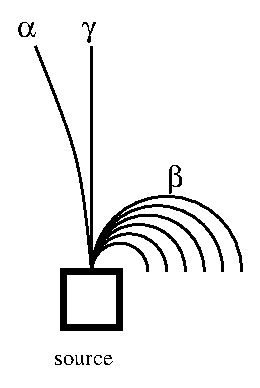
\includegraphics[clip]{1993phy4-1.eps}}
  \end{center}}

  \end{subsubquestions}


\end{subquestions}
\end{question}
\begin{answer}{専攻 問題4}{}
\def\Bracket#1#2#3{\langle{#1}|{#2}|{#3}\rangle}
\def\Mean#1{\langle{#1}\rangle}
\def\Vec#1{\vec{#1}\,}

\def\mX{m\ssub{X}}
\def\mY{m\ssub{Y}}
\def\mA{m\ssub{\alpha}}
\def\mG{m\ssub{\gamma}}
\def\pX{\vec{p}\ssub{X}}
\def\pY{\vec{p}\ssub{Y}}
\def\pA{\vec{p}\ssub{\alpha}}
\def\pG{\vec{p}\ssub{\gamma}}


\begin{subanswers}
\SubAnswer
  \begin{subsubanswers}
  \SubSubAnswer
    2つの核子系に対する完全な波動関数は
    $f(\Vec{r},\Vec{s}_1,\Vec{s}_2,\Vec{\tau}_1,\Vec{\tau}_2)$
    と書かれる。

    \begin{tabular}{ccl}
      $\Vec{r}$ &:& 2核子の相対座標 \\
      $\Vec{s}_1,\Vec{s}_2$ &:& 2核子のspin空間座標 \\
      $\Vec{\tau}_1,\Vec{\tau}_2$&:& 2核子のisospin空間座標
    \end{tabular}

    ここでハミルトニアンにおける異なる種類の自由度間の相互作用が
    無視できると、
%
    \[ f = f_{r}(\Vec{r})f_{\sigma}f_{\tau} \]	
%
    と分解できる。\\
%
    核子はfermionなので、波動関数は座標の交換について反対称で
    なければいけない。したがって、
%
    \begin{itemize}
    \item p-n系        $S_{1}$状態にあるものは $f_{r}(\Vec{r})$と$f_{\sigma}$が対称。従ってisospin \ $f_{\tau}$ は反対称。
    \item p-p系,n-n系  isospin \, $f_{\tau}$ は対称。従って $f_{r}(\Vec{r})f_{\sigma}$は反対称。
    \end{itemize}
%
    となる。また、軌道角運動量$L$の状態では空間部分は
    $f_{r}(-\Vec{r})=(-1)^L f_{r}(\Vec{r})$である。\\
%
    以上のことを考えた結果、下表のようになる。

    \begin{tabular}{|c|c|c|c|}\hline
                  & d         & \multicolumn{2}{c|}{p-p,n-n} \\ \hline
     スピン       & 対称      & 対称        & 反対称    \\ \hline
     アイソスピン & 反対称    & 対称        & 対称      \\ \hline
     空間部分(L)  & 対称(L偶) & 反対称(L奇) & 対称(L偶) \\ \hline    
    \end{tabular}

    よって、p-p, n-n ,p-n系でspin-parityは一緒ではありえない。
    従って、矛盾は起こらない。

  \SubSubAnswer
    \begin{itemize}
    \item 磁気モーメントが $\mu_{p}+\mu_n\neq\mu_d$となっていること。\\
          軌道角運動量が$0$でない状態が混ざっているとすれば、
          その効果による磁気モーメントが生まれるから。

    \item 電気的四重極モーメントが0でないこと。\\
	  $s$軌道は電気的四重極モーメントを持たないが、空間的に
          クローバー型をした$d$軌道波動関数は四重極モーメントを
          持つから。
    \end{itemize}

  \SubSubAnswer
    $\Mean{\Vec{J}\cdot\Vec{I}}$を$F,J,I$で表す。
%
    \[ \Vec{F} = \Vec{J}+\Vec{I} \hspace{10mm}%
       \Vec{F}^2 = \Vec{J}^2+\Vec{I}^2+2\Vec{J}\cdot\Vec{I} \]
%
    従って
%
    \begin{eqnarray*}
      \Mean{\Vec{J}\cdot\Vec{I}}%
      &=& \Bracket{FIJ}{\Vec{J}\cdot\Vec{I}}{FIJ}%
       =  \Bracket{FIJ}{\frac{1}{2}(\Vec{F}^2-\Vec{J}^2-\Vec{I}^2)}{FIJ} \\
      &=& \frac{1}{2}[F(F+1)-J(J+1)-I(I+1)]
    \end{eqnarray*}
%
    次に、重水素の分裂エネルギーを求める。(以下で陽子、重陽子の$g$
    因子をそれぞれ$g_p$、$g_d$、磁気能率を$\mu_{p}$、$\mu_{d}$と
    記す。)\\
%
    前の式に電子のスピン$J=1/2$を代入すると、
%
    \[ \Mean{\Vec{J}\cdot\Vec{I}}%
       = \frac{1}{2}\left[F(F+1)-\frac{3}{4}-I(I+1)\right]
       = \frac{1}{2}\left\{\begin{array}{cc}
                     I   & (F=I+1/2) \\
                    -I-1 & (F=I-1/2) \end{array}\right. \]
%
    となるので、超微細構造の分裂は、
%
    \[ \IDelta E%
       = \alpha g_{I}\cdot\IDelta(\Mean{\Vec{J}\cdot\Vec{I}})%
       = \frac{\alpha g_{I}}{2}(2I+1) \]
%
    である。
\newpage
    次に、重水素の準位の分裂を求める。\\
    まず、水素の場合、核のスピン$I=1/2$であるから、準位の分裂は、
%
    \[ \IDelta E%
       = \frac{\alpha g_{p}}{2}\cdot(2\cdot\frac{1}{2}+1)%
       = \alpha g_{p}%
       = 5.9\Keta{-6}\Unit{eV} \]
%
    である。次に重陽子は、スピン$I=1$である。また、原子核の磁気能率の
    大きさの定義が「磁気能率演算子$\Vec{\mu}_{I}=g_{I}\mu_{N}\Vec{I}$
    の$z$成分の磁気量子数$m_{I}=I$の状態での期待値」であるので、陽子、
    重陽子それぞれの磁気能率は
%
    \[ \mu_{p} = g_{p} \mu_{N} \cdot I%
               = g_{p} \mu_{N}\cdot\frac{1}{2} =2.793 \mu_{N}  \]
    \[ \mu_{d} = g_{d} \mu_{N} \cdot I
               = g_{d} \mu_{N} \cdot 1  = 0.857 \mu_{N}\]
%
    となる。従って、重水素の準位の分裂は、
%
    \begin{eqnarray*}
      \IDelta E%
        &=& \frac{\alpha g_{d}}{2} \cdot(2\cdot1+1)%
         =  \alpha g_{d}\cdot \frac{3}{2}%
         =  (\alpha g_{p})\cdot\frac{g_{d}}{g_{p}}\cdot\frac{3}{2} \\
        &=& (5.9\Keta{-6})\times\frac{0.857}{2\times 2.793}\times%
            \frac{3}{2}
        \simeq 1\Keta{-6} \Unit{eV}
    \end{eqnarray*}

  \end{subsubanswers}


\SubAnswer
  \begin{subsubanswers}
  \SubSubAnswer
    図からわかること。
%
    \begin{itemize}
    \item $\gamma$線は電荷をもたない。
    \item $\alpha$線と $\beta$線は互いに反対の電荷をもつ
    \item $\alpha$線が$+2$の電荷をもつことから、磁場は
          紙面の表から裏にむけてかかっている。
    \item $\alpha$線は単一のエネルギーをもつのに対し、
          $\beta$線はさまざまなエネルギーをもつ。
    \item $|q|=mv/rB=p/rB$なので、$\alpha$線は運動量が大きく、
          $\beta$線は小さい。
    \end{itemize}
%
    ただし、$v$ は線源から出る時の速度、$p$は運動量、$|q|$は電荷、
    $r$は軌跡の曲率半径、$B$は磁場をそれぞれ表している。

  \SubSubAnswer
    $Q$値が核子の静止質量より十分小さいので、$\gamma$線以外には
    非相対論的近似をする。\\

    {\bf $\alpha$崩壊}\\
%
    始状態の原子核を$X$、終状態を$Y$とすると、崩壊の図式は以下の
    ようになる。
%
    \[X\longrightarrow Y+\alpha \]
%
    各粒子の質量を$\mX,\mY,\mA,\mG$、運動量を $\pX,\pY,\pA,\pG$
    と表すことにすれば、エネルギーと運動量の保存則より、
%
    \begin{eqnarray}
      \mX &=& \mY+\mA+\frac{\pA^2}{2\mA}+\frac{\pY^2}{2\mY}%
      \eqname{1}\\
      \pX &=& \pY+\pA = 0 \eqname{2}
    \end{eqnarray}
%
    が得られる。\\
    式\eqhref{2}から、$\pY^2=\pA^2$が得られ、これと式\eqhref{1}より、
    $Q$を計算すると、
%
    \[ Q = \mX-\mY-\mA%
         = \frac{\pA^2}{2\mA}+\frac{\pY^2}{2\mY}%
         = \frac{\pY^2}{2\mY}
           \left(1+\frac{\mY}{\mA}\right) \]
%
    となる。これから求める反跳エネルギー$\pY^2/2\mY$を求めることが
    できて、
%
    \[ \frac{\pY^2}{2\mY}%
         = \frac{Q}{1+\mY/\mA}%
         = \frac{5\Unit{MeV}}{1+196/4}%
         = 0.1\Unit{MeV} \]
%
    となる。

\newpage
    {\bf $\gamma$崩壊}\\
%
    $\alpha$崩壊の場合と同様にして崩壊の図式は、
%
    \[ X \longrightarrow Y+\gamma \]
%
    エネルギー運動量保存則は、
%
    \begin{eqnarray}
      \mX &=& \mY+|\pG|+\frac{\pY^2}{2\mY} \eqname{3} \\
      \pX &=& \pG+\pY = 0 \eqname{4}
    \end{eqnarray}
%
    である。式\eqhref{3},\eqhref{4}から、
%
    \[ Q = \mX-\mY%
         = |\pG|+\frac{\pY^2}{2\mY}%
         = |\pY|+\frac{\pY^2}{2\mY} \]
%
    となり、これを二次方程式の形に直して、
%
    \[ |\pY|^2+2\mY|\pY|-2\mY Q=0 \hspace{15mm}
       \Yueni |\pY|=-\mY+\sqrt{\mY^2+2\mY Q} \]
%
    となる。ただし、第二項の符号が$+$になっているのは、
    $|\pY|>0$による。$\mY\gg Q$を用いてこれを計算すると、
%
    \[ |\pY| = -\mY+\mY\sqrt{1+\frac{2Q}{\mY}}%
             \simeq -\mY+\mY\left(1+\frac{Q}{\mY}\right)%
             = Q \]
%
    となる。従って反跳エネルギーは、
%
    \[ \frac{\pY^2}{2\mY}%
          = \frac{Q^2}{2\mY}%
          = \frac{1}{2\cdot200\cdot940}%
          \simeq 3\Unit{eV} \]
%
    となる。


  \SubSubAnswer
    $\beta$崩壊は終核と$e^-$と$\bar{\nu_e}$が出てくる三体崩壊で
    あるから、エネルギー運動量保存則からでは、電子の持つエネルギーや
    運動量の値は決まらないからである。\\
    $\bar{\nu_e}+p\rightarrow e^{+}+n$で生じた$e^{+}$は、対消滅
    ($e^{+}+e^{-}\rightarrow2\gamma$)で生じる$\gamma$線を測定すること
    で、nはそれが核に捕獲されたとき生じる(n,$\gamma$)反応の$\gamma$線
    を測定することで検出される。後者の$\gamma$線は前者よりもおくれて
    発生するので、両者を遅延同時計数法により測定する。 \\
    なお、この実験では、単一の$\bar{\nu_e}$と$p$との反応ではなく、関
    係のない核子が多数存在するので、$e^+$と$n$を直接検出したところで、
    この反応を検証したことにならないことに注意。

  \end{subsubanswers}
\end{subanswers}
\end{answer}


\end{document}
